\documentclass[12pt,a4paper,english]{paper}
\usepackage{fontspec}
\usepackage[T1]{fontenc}
\usepackage[utf8]{inputenc}
\usepackage[left=0.65in,right=0.65in,top=2cm,bottom=1in]{geometry}
\usepackage{multirow}
\usepackage{hyperref}
\usepackage{graphicx}
\usepackage{bm}
\usepackage[usenames,dvipsnames]{color}
\usepackage{booktabs}
\usepackage{fancyhdr}
\usepackage[most]{tcolorbox}
\usepackage{changepage}
\usepackage[square,sort,comma,numbers]{natbib}
\usepackage{amsmath}
\usepackage{amssymb}
\usepackage{eucal}
\usepackage[]{minted}
\usepackage{latexsym}
\usepackage{indentfirst}
\usepackage[ruled,vlined]{algorithm2e}
\usepackage[english]{babel}
\usepackage[autostyle, english = american]{csquotes}
\usepackage[default]{lato}
\usepackage{FiraMono}
\usepackage{caption}
\usepackage{lipsum}

\MakeOuterQuote{"}

\def \courseNumber {CS6630}
\def \courseName {Secure Processor Microarchitecture}
\def \assignmentName {Assignment 3}
\def \myName {Arjun Menon V, Akilesh Kannan}
\def \rollNumber {EE18B104, EE18B122}

\setlength{\headheight}{14pt}

\pagestyle{fancy}
\fancyhf{}
\rhead{\assignmentName}
\lhead{\courseNumber: \courseName}
\cfoot{\thepage}

% \linespread{1.2}

\definecolor{blue(ryb)}{rgb}{0.01, 0.28, 1.0}
\definecolor{green(ryb)}{rgb}{0.28, 1.0, 0.01}
\definecolor{red(ryb)}{rgb}{1.0, 0.01, 0.28}
\definecolor{black(ryb)}{rgb}{0, 0, 0}
\definecolor{gray(ryb)}{rgb}{0.75, 0.75, 0.75}
\definecolor{orange}{RGB}{255,155,0}
\definecolor{formalblue}{rgb}{0.95,0.95,1}
\definecolor{formalred}{rgb}{1,0.95,0.95}

\newenvironment{colorboxed}[4][gray]{
\begin{tcolorbox}[colback=#1!3!white,colframe=#1(ryb)!50!black,title=\textbf{#2 #3},#4]
}{
\end{tcolorbox}
}

\newenvironment{warning}{%
  \def\FrameCommand{%
    \hspace{1pt}%
    {\color{red}\vrule width 2pt}%
    {\color{formalred}\vrule width 4pt}%
    \colorbox{formalred}%
  }%
  \MakeFramed{\advance\hsize-\width\FrameRestore}%
  \noindent\hspace{-4.55pt}% disable indenting first paragraph
  \begin{adjustwidth}{7pt}{}%
  \vspace{2pt}\vspace{2pt}%
}
{%
  \vspace{2pt}\end{adjustwidth}\endMakeFramed%
}

\newenvironment{results}{%
  \def\FrameCommand{%
    \hspace{1pt}%
    {\color{blue}\vrule width 2pt}%
    {\color{formalblue}\vrule width 4pt}%
    \colorbox{formalblue}%
  }%
  \MakeFramed{\advance\hsize-\width\FrameRestore}%
  \noindent\hspace{-4.55pt}% disable indenting first paragraph
  \begin{adjustwidth}{7pt}{}%
  \vspace{2pt}\vspace{2pt}%
}
{%
  \vspace{2pt}\end{adjustwidth}\endMakeFramed%
}

\begin{document}
\thispagestyle{empty}
\vspace{-4.5cm}

\hspace*{-\parindent}
\begin{minipage}{0.65\textwidth}
\fontsize{22pt}{10pt}\selectfont\textbf{\assignmentName}\\[1mm]
\Large
\textit{\courseNumber: \courseName}\\[5mm]
\Large \myName \\[1mm]
\normalsize \rollNumber \\
\end{minipage}\hfill% push everything to the right
\raisebox{-13mm}{
\includegraphics[scale=.28]{logo.pdf}}

\hrule \hrule
\medskip

\section{Single-Fault Attack on AES-128}

\begin{warning}
The attack implemented here is adapted from this work \cite{10.1007/978-3-642-21040-2_15}.
\end{warning}

\subsection{Approach}
In order to break the secret key for AES, we only need to get one of the round keys. In this case, we can easily get the last round key through some simple analysis when a fault is introduced in the $8^{\text{th}}$, before the {\fontfamily{cmr}\selectfont MixColumns} step.

\begin{figure}[H]
    \centering
    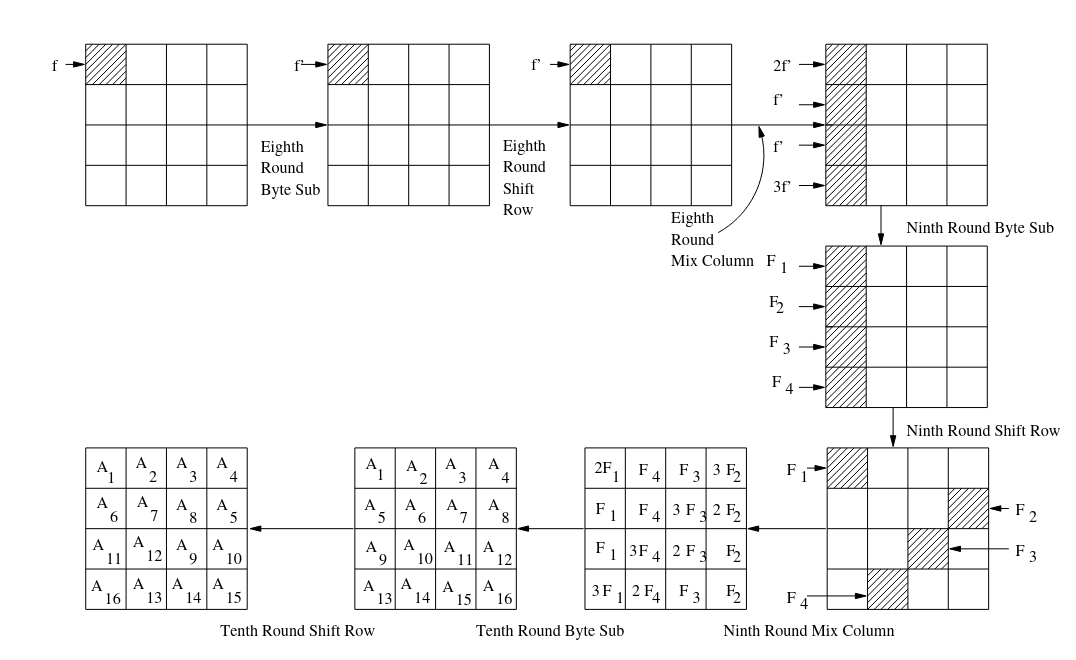
\includegraphics[scale=0.4]{FaultProp.png}
    \caption{Propagation of $8^{\text{th}}$ round fault \cite{10.1007/978-3-642-21040-2_15}}
    \label{fig:fault_prop}
\end{figure}

Let us assume that the fault in $8^{\text{th}}$ round is introduced at position 0. We can then trace the propagation of the fault through the rounds as shown in Fig.\ref{fig:fault_prop}.

At the end of $9^{\text{th}}$ round (after  {\fontfamily{cmr}\selectfont MixColumns}), we arrive at the following sets of equations, each involving 4 bytes  of the round 10 key $\text{\textit{K}}_{10}$:
\begin{gather*}
    2F_1 = S^{-1}(x_{0} \oplus k_{0}) \oplus S^{−1}(x_{0}' \oplus k_{0})\\
    F_1 = S^{−1}(x_{13} \oplus k_{13}) \oplus S^{−1}(x_{13}' \oplus k_{13})\\
    F_1 = S^{−1}(x_{10} \oplus k_{10}) \oplus S^{−1}(x_{10}' \oplus k_{10})\\
    3F_1 = S^{−1}(x_{7} \oplus k_{7}) \oplus S^{−1}(x_{7}' \oplus k_{7})
\end{gather*}
\begin{gather*}
    2F_4 = S^{-1}(x_{11} \oplus k_{11}) \oplus S^{−1}(x_{11}' \oplus k_{11})\\
    F_4 = S^{−1}(x_{4} \oplus k_{4}) \oplus S^{−1}(x_{4}' \oplus k_{4})\\
    F_4 = S^{−1}(x_{1} \oplus k_{1}) \oplus S^{−1}(x_{1}' \oplus k_{1})\\
    3F_4 = S^{−1}(x_{14} \oplus k_{14}) \oplus S^{−1}(x_{14}' \oplus k_{14})
\end{gather*}
\begin{gather*}
    2F_3 = S^{-1}(x_2 \oplus k_2) \oplus S^{−1}(x_2' \oplus k_2)\\
    F_3 = S^{−1}(x_{8} \oplus k_{8}) \oplus S^{−1}(x_{8}' \oplus k_{8})\\
    F_3 = S^{−1}(x_{15} \oplus k_{15}) \oplus S^{−1}(x_{15}' \oplus k_{15})\\
    3F_3 = S^{−1}(x_{8} \oplus k_{8}) \oplus S^{−1}(x_{8}' \oplus k_{8})
\end{gather*}
\begin{gather*}
    2F_2 = S^{-1}(x_9 \oplus k_9) \oplus S^{−1}(x_9' \oplus k_9)\\
    F_2 = S^{−1}(x_{3} \oplus k_{3}) \oplus S^{−1}(x_{3}' \oplus k_{3})\\
    F_2 = S^{−1}(x_{6} \oplus k_{6}) \oplus S^{−1}(x_{6}' \oplus k_{6})\\
    3F_2 = S^{−1}(x_{12} \oplus k_{12}) \oplus S^{−1}(x_{12}' \oplus k_{12})
\end{gather*}

where, $S()$ denotes the SBOX operation, $S^{-1}()$ denotes it's inverse operation, $x_i$ denotes the $i^{\text{th}}$ byte of the correct ciphertext and $x_i'$ denotes the same in the faulty ciphertext. The byte ordering followed is column-major.\\

% \begin{table}[H]
% \centering
% \begin{tabular}{|c|c|c|c|}
% \hline
% $x_0$ & $x_4$ & $x_8$    & $x_{12}$ \\ \hline
% $x_1$ & $x_5$ & $x_9$    & $x_{13}$ \\ \hline
% $x_2$ & $x_6$ & $x_{10}$ & $x_{14}$ \\ \hline
% $x_3$ & $x_7$ & $x_{11}$ & $x_{15}$ \\ \hline
% \end{tabular}%
% \caption*{Ciphertext Byte order}
% \label{tab:text-order}
% \end{table}

As shown in \cite{10.1007/978-3-642-21040-2_15}, we get $\sim256$ solutions for each of the 4 sets of equations, thus resulting in $2^{32}$ possible solutions for $\text{\textit{K}}_{10}$. Since, we do not know the position of the induced fault, we repeat this analysis assuming the fault is induced independently at each of the 16 bytes, resulting in $\sim4096$ solutions for each of the 4-byte subkeys and a total of $2^{36}$ possible $\text{\textit{K}}_{10}$ values.

While \cite{10.1007/978-3-642-21040-2_15} proposes a $2^{\text{nd}}$ step in the attack, exploiting the relationship between $9^{\text{th}}$ and $10^{\text{th}}$ round keys to narrow this search space down, we have decided to take a different approach, making use of multiple CT-FCT pairs.

We repeat the above experiment on another CT-FCT pair, and find common solutions for each of the 4-byte subkeys with the previous pair.

\textit{Note that we do not search over the entire $2^{36}$ possibilities for $\text{\textit{K}}_{10}$, but rather only search among the $\sim4096$ solutions for each of the 4-byte subkeys} - This allows us to find $\text{\textit{K}}_{10}$ rather quickly by piecing together the 4 partial subkeys.

After obtaining $\text{\textit{K}}_{10}$, we can get the secret key and other round keys by backtracking through the {\fontfamily{cmr}\selectfont KeySchedule} algorithm.

\subsection{Results}
% Please add the following required packages to your document preamble:
% \usepackage{multirow}
% \usepackage{graphicx}
\begin{table}[H]
\centering
\resizebox{\columnwidth}{!}{%
\begin{tabular}{ccl}
\hline
\textbf{Parameter}                       & \multicolumn{2}{c}{\textbf{Value}}                                                                    \\ \hline
\multicolumn{1}{c|}{Retrieval Time}      & \multicolumn{2}{c}{2min 3sec}                                                                         \\ \hline
\multicolumn{1}{c|}{No. of CT-CT' pairs} & \multicolumn{2}{c}{2}                                                                                 \\ \hline
\multicolumn{1}{c|}{Secret Key}          & \multicolumn{2}{c}{{[}107 142 167 187 226 167 118 199  34 185 173  84  32 102  14 150{]}}             \\ \hline
\multicolumn{1}{c|}{\multirow{10}{*}{Round Keys}} & \multicolumn{1}{c|}{Round 1} & {[} 88  37  55  12 136 152 236  57 230 255  99  70 174 112 245 204{]} \\ \cline{2-3}
\multicolumn{1}{c|}{}                             & \multicolumn{1}{c|}{Round 2}  & {[}  9 195 124 232 137 182 252 162  65 177 211 124  45 184 147 220{]} \\ \cline{2-3}
\multicolumn{1}{c|}{}                             & \multicolumn{1}{c|}{Round 3}  & {[}101  31 250  48 196 118 209 166  93 137 237  88  97  31 198 182{]} \\ \cline{2-3}
\multicolumn{1}{c|}{}                             & \multicolumn{1}{c|}{Round 4}  & {[}165 171 180 223 194  20  92  56 120 115 167  95 221 144 154 121{]} \\ \cline{2-3}
\multicolumn{1}{c|}{}                             & \multicolumn{1}{c|}{Round 5}  & {[}197  19   2  30 100 105  43  74  59 138  86 137  63 238  43 222{]} \\ \cline{2-3}
\multicolumn{1}{c|}{}                             & \multicolumn{1}{c|}{Round 6}  & {[}237 226  31 107  49 241 235  53 252  43 191  31 143  31  35  30{]} \\ \cline{2-3}
\multicolumn{1}{c|}{}                             & \multicolumn{1}{c|}{Round 7}  & {[} 45 196 109  24 233 237 215 152 226 126 177  89  23 236 235 213{]} \\ \cline{2-3}
\multicolumn{1}{c|}{}                             & \multicolumn{1}{c|}{Round 8}  & {[}227  45 110 232 248  53  72   3 163 232 227  34  29 119 250  70{]} \\ \cline{2-3}
\multicolumn{1}{c|}{}                             & \multicolumn{1}{c|}{Round 9}  & {[} 22   0  52  76 191  86  80  42 171  89 176 199 127 188  29 128{]} \\ \cline{2-3}
\multicolumn{1}{c|}{}                             & \multicolumn{1}{c|}{Round 10} & {[}115 164 249 158  48  31 201  33 175 153 109  58   6  82  33   0{]} \\ \hline
\end{tabular}%
}
\caption{Results}
\label{tab:summary}
\end{table}

\subsection{Code}
\begin{colorboxed}{Password cracker script}{}{breakable}
    \inputminted[baselinestretch=0.85,breaklines,fontsize=\footnotesize]{python}{../src/dfa_8.py}
\end{colorboxed}
%Beginning References. Don't add any text beyond this.
%------------------------------------------

%\newpage %sending References to the last page

\bibliography{ref}
\bibliographystyle{acm}
\end{document}
